\section{\textbf{WAHRSCHEINLICHKEITSTHEORIE} - Ereignisse und Wahrscheinlichkeiten}
\subsection{Zufallsereignisse}
Der Ausgangspunkt jeder wahrscheinlichkeitstheoretischen Betrachtung ist ein Zufallsvorgang oder Zufallsexperiment (Würfeln, prüfen eines Werkstücks). Einen Zufallsvorgang zeichnet aus, dass es mehrere, \emph{sich gegenseitig ausschließende} Ergebnisse gibt, von dem genau eines Eintreten wird, wobei nicht bekannt ist welches. Die \emph{möglichen} Ergebnisse eines Zufallsvorgang werden mit $\omega$ und die Menge aller Ergebnisse d.h. der \emph{Ergebnisraum} werden als $\Omega$ bezeichnet. Beim Einmaligen Würfeln kann $\omega$  z.B. $\omega = \{2\}$ sein, während $\Omega = \{1, 2, 3, 4, 5, 6\}$ ist. Wenn man beim Würfeln eine 5 oder 6 benötigen um zu gewinnen, ist man daran interessiert, ob das
Ergebnis des Würfelwurfes in einer bestimmten Teilmenge von $\Omega$ liegt, konkret in der Menge $\{5, 6\}$. Diese Teilmengen nennt man \emph{(Zufalls-)Ereignisse} und man sagt, dass ein Ereignis $A \subset \Omega$ eintritt, wenn das Ergebnis $\omega$ des Zufallsvorgang ein Element von A is. Die einelementigen Teilmengen $\{\omega\}$ von $\Omega$ nennt man auch \emph{Elementareereignisse}.\\\\
\textbf{Mengenlehre und wahrscheinlichkeitstheoretische Interpretation}: \emph{Kommutativgesetz}: $A \cap  B = B \cap A$. \emph{Assoziativgesetz}: $(A \cap B ) \cap C = A \cap (B \cap C)$. \emph{Distributivgesetz}: $(A \cup B) \cap C = (A \cap C) \cup (A \cap C)$. \emph{De Morgansche Regel}: $\overline{(A \cap B)} = \bar{A} \cup \bar{B}$ (geht auch, wenn man $\cap$ und $\cup$ vertauscht)\\\\
\textbf{Ereignisfelder}: Die Menge aller Ergebnisse bezeichnet man als \emph{Ereignisfeld} $\mathcal{F}$. Wenn der Ergebnisraum $\Omega$ endlich oder abzählbar unendlich ist, ist die Potenzmenge $\mathcal{P}(\Omega)$ das üblicherweise betrachtete Ereignisfeld. Ist $\Omega$ überabzählbar können als Ereignisfelder nur $\sigma$-Algebren betrachtet werden. Diese sind definiert durch: $\Omega \in \mathcal{F}$,\,\,\,$A \in \mathcal{F} \Rightarrow \bar{A} \in \mathcal{F}$,\,\,\,abzählbar viele Ereignisse $A_1, A_2, ... \in \mathcal{F} \Rightarrow \cup_{i=1}^\infty A_i \in \mathcal{F}$

\subsection{Laplace-Wahrscheinlichkeiten und Kombinatorik}
\begin{wrapfigure}{r}{0.4\textwidth}
    \vspace{-6mm}
    \centering
    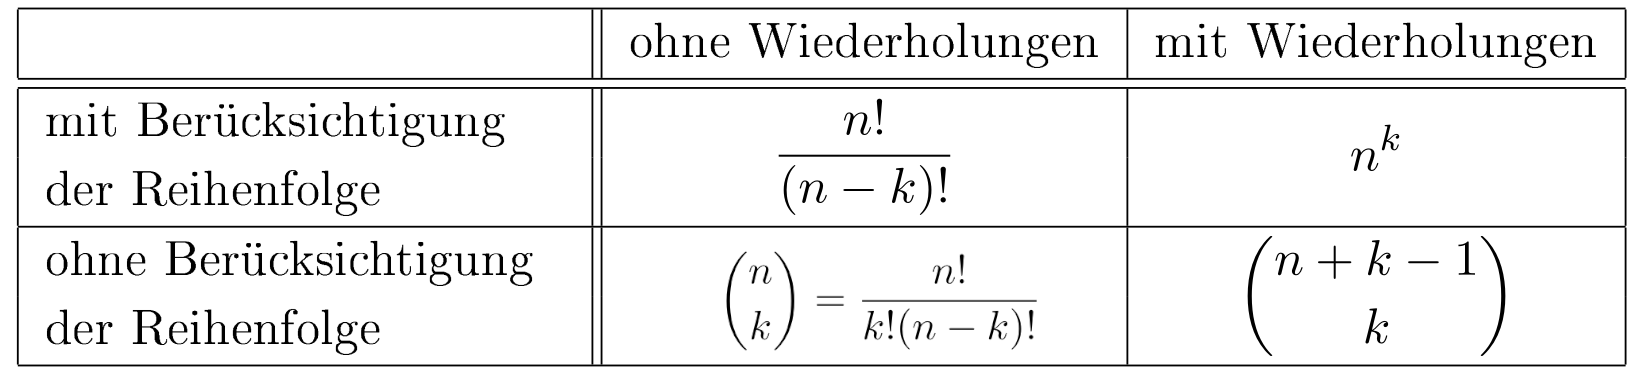
\includegraphics[width=0.4\textwidth]{images/wiederholung_kombinatorik.png}
    \caption{Kombinatorik Wiederholung}
    \vspace{-6mm}
    \label{fig:}
\end{wrapfigure}
\textbf{Laplace-Wahrscheinlichkeit}: $P(A) = \frac{\text{Anzahl der für $A$ günstigen Ergebnisse}}{\text{Anzahl aller möglichen Ergebnisse}} = \frac{|A|}{|\Omega|}$. Bsp. die Wahrscheinlichkeit eine ungerade Zahl zu würfeln: $P(A) = \frac{|\{1,3,5\}|}{|\{1,2,3,4,5,6\}|} = \frac{3}{6} = \frac{1}{2}$

\textbf{Permutation}: Anordnen von n unterscheidbaren Objekten: $n \cdot (n-1) \cdot (n-2) ... = \Pi_{i=1}^n i = n!$. Bsp: Sitzordnung an einem Tisch.\,\,\,\,\textbf{Variation ohne Wiederholungen}: Möglichkeiten k aus n unterscheidbaren Objekten \emph{mit} Berücksichtigung der Reihenfolge auszuwählen. Formel 1 Siegertreppchen Anordnungen bei 20 Teilnehmern.\,\,\,\,\textbf{Variation mit Wiederholungen}: Bsp. k mal ziehen aus n Möglichkeiten. Bsp: Kombinationen bei Passwörtern.\,\,\,\,\textbf{Kombination ohne Wiederholungen} Ziehen von k aus n Objekten. Die Reihenfolge spielt keine Rolle. Bsp: \hlc{Lotto} 6 aus 49.\,\,\,\,\textbf{Kombination mit Wiederholungen}: Die Anzahl Kombinationen beim Auswählen von k Objekten aus n unterscheidbaren Objekten.
\subsection{Wahrscheinlichkeitsmaße}
\textbf{Definition Wahrscheinlichkeitsmaß}: Es sei $\Omega$ der Ergebnisraum eines Zufallsvorgangs und $\mathcal{F}$ ein Ereignisfeld über $\Omega$. Eine Abbildung $P$ die jedem Ereignis $A \in \mathcal{F}$ eine reelle Zahl zuordnet: $P: \mathcal{F} \rightarrow \mathds{R}$ mit $A \mapsto P(A)$ nennt man \emph{Wahrscheinlichkeitsmaß} auf $\mathcal{F}$ wenn sie die \hlc{Axiome von Kolmogoroff} erfüllt: \textbf{K1} $P(A) \ge 0$ (Nichtnegativität).\,\,\,\,\textbf{K2} $P(\Omega) = 1$ (Normierung).\,\,\,\,\textbf{K3} Falls $A \cap B = \emptyset$, so ist $ (A \cup B) = P(A) + P(B)$ (Additivität).\\
Daraus folgen folgende Rechenregel:\,\,\,\,(\textbf{i}) $0 \le P(A) \le 1$.\,\,\,\,(\textbf{ii}) $P(\emptyset) = 0$.\,\,\,\,(\textbf{iii}) $P(A) \le P(B)$, falls $A \subset B$.\,\,\,\,(\textbf{iv}) $P(\bar{A}) = 1 - P(A)$.\,\,\,\,(\textbf{v}) $P(A_1\cup ... \cup A_k) = P(A_1) + ... + P(A_k)$ falls $A_1, ..., A_k$ paarweise disjunkt. $\Rightarrow$ $P(A) = \sum_{w \in A}P(\{\omega\}.$\,\,\,\,(\textbf{vi}) $P(B \backslash A) = P(B) - P(A \cap B)$.\,\,\,\,(\textbf{vii}) $P(A\cup B) = P(A) + P(B) - P(A \cap B)$ (Additionssatz)
\subsection{Bedingte Wahrscheinlichkeiten und unabhängige Ereignisse}
Die Wahrscheinlichkeit eines Ereignisses ändert sich möglicherweise, wenn wir zusätzlich Information in Form des Eintritts eines anderen Ereignisses erhalten. Wahrscheinlichkeit für Pünktlichkeit sinkt bei Stau. Die Definition der \hlc{bedingten Wahrscheinlichkeit} ergibt sich hierbei Analog zur relativen Häufigkeitsverteilung: \hlcm{$P(A|B) = \frac{P(A \cap B)}{P(B)}$}. Bsp: Wie hoch ist die Wahrscheinlichkeit eine 6 zu würfeln unter der Bedingung, dass die gewürfelte Zahl gerade ist? Antwort: $P(A|B) = \frac{P(\{6\} \cap \{2,4,6\})}{P(\{2,4,6\})} = \frac{1/6}{3/6} = \frac{1}{3}$\\
\begin{wrapfigure}{l}{0.25\textwidth}
    \vspace{-6mm}
    \centering
    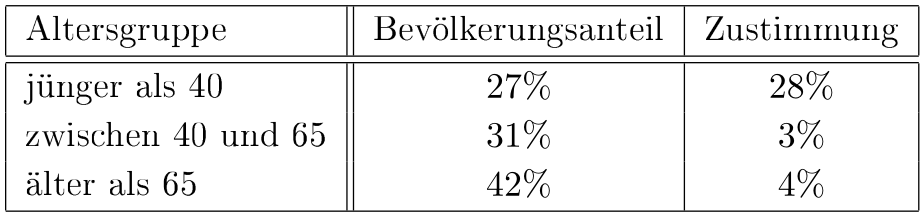
\includegraphics[width=0.25\textwidth]{images/beispiel_wahl_satz_der_tot_wahscheinlichkeit.png}
    \caption{Eine Partei hat analysiert, wie ihre Demographie ist.}
    \vspace{-5mm}
    \label{fig:pool_total}
\end{wrapfigure}
Der \hlc{Produktsatz} garantiert, dass für zwei Ergebnisse $A$ und $B$ mit $P(B) > 0$ gilt: \hlcm{$P(A \cap B) = P(B) \cdot P(A|B)$}. Diese Aussage gilt auch im allgemeinen für $A_1, ..., A_n$ mit $P(A_1 \cap ... \cap A_n) > 0$:\\$P(\cap_{i=1}^nA_i) = P(A_1) \cdot P(A_2|A_1) \cdot P(A_3|A_1 \cap A_2) \cdot P(A_n|A_1 \cap ... \cap A_{n-1}) = P(A_1) \cdot \Pi_{i=2}^n P(A_i|A_1 \cap ... \cap A_{i-1})$. \hlc{Stochastiche Unabhängikeit} bedeutet wenn sich die Wahrscheinlichkeit eines Ereignisses $A$ beim Eintritt eines anderen Ereignisses $B$ \emph{nicht} ändert. Sprich $P(A|B) = P(A)$. Somit gild dann mit dem Produktsatz $P(A \cap B) = P(B) \cdot P(A | B) = P(B) \cdot P(A)$. Dies gilt Analog für $n$ Ereignisse. \hlc{Satz der totalen Wahrscheinlichkeit}: Sei $A_1, ..., A_n$ eine disjunkte Zerlegung des Ereignisraums $\omega$ mit $P(A_j) > 0$, $j = 1, ..., n$. Dann gilt für ein weiteres Ereignis $B$: \hlcm{$P(B) = \sum_{j=1}^nP(B|A_j) \cdot P(A_j)$}. Bsp Wahl (vgl \cref{fig:pool_total}) Welchen Stimmanteil hat die Partei insgesamt bekommen? Antwort: $P(B) = \sum_{j=1}^3 = P(B|A_j) \cdot P(A_j) = 0.28 \cdot 0.27 + 0.03 \cdot 0.031 + 0.04 \cdot 0.42 = 0.1017$. \hlc{Satz von Bayes}: Sei $A_1, ..., A_n$ eine disjunkte Überdeckung des Ereignisses $B$ und $P(A_j) > 0$ sowie $P(B|A_j) > 0$ für mindestens ein $j = 1, ..., n$. Dann gilt: \hlcm{$P(A_j|B) = \frac{P(B|A_j) \cdot P(A_j)}{P(B)} = \frac{P(B|A_j) \cdot P(A_j)}{\sum_{i=1}^nP(B|A_i) \cdot P(A_i)}, j = 1, ..., n$}. Dieser Satz überträgt die \emph{a-priori} Wahrscheinlichkeit $P(A_j)$ in eine \emph{a-posteriori} Wahrscheinlichkeit $P(A_j|B)$. Bsp. Wie groß ist die Wahrscheinlichkeit, dass ein Wähler zur Gruppe \glqq jünger als 40\grqq\, gehört? Antwort: ($P(B)$ wurde mit Satz der tot. Wahrscheinlichkeit berechnet) $P(A_1|B) = \frac{P(B|A_1) \cdot P(A_1)}{P(B)} = \frac{0.28 \cdot 0.27}{0.1017}$
\section{Zufallsvariablen}
\begin{wrapfigure}{r}{0.2\textwidth}
    \vspace{-10mm}
    \centering
    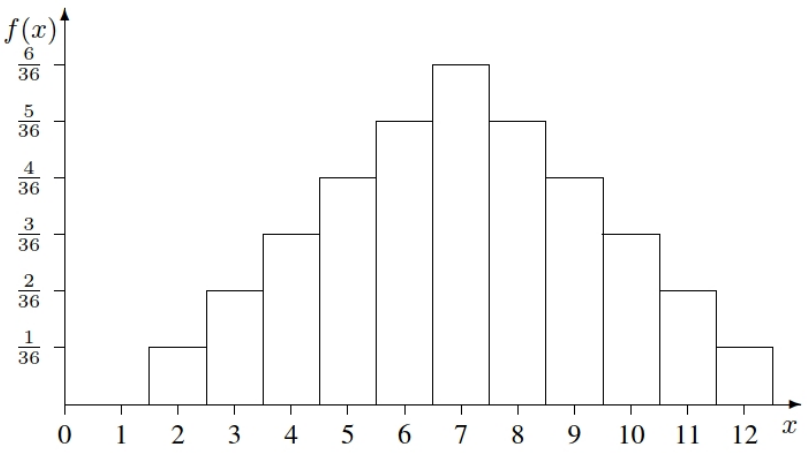
\includegraphics[width=0.2\textwidth]{images/5.1_f_augensumme.png}
    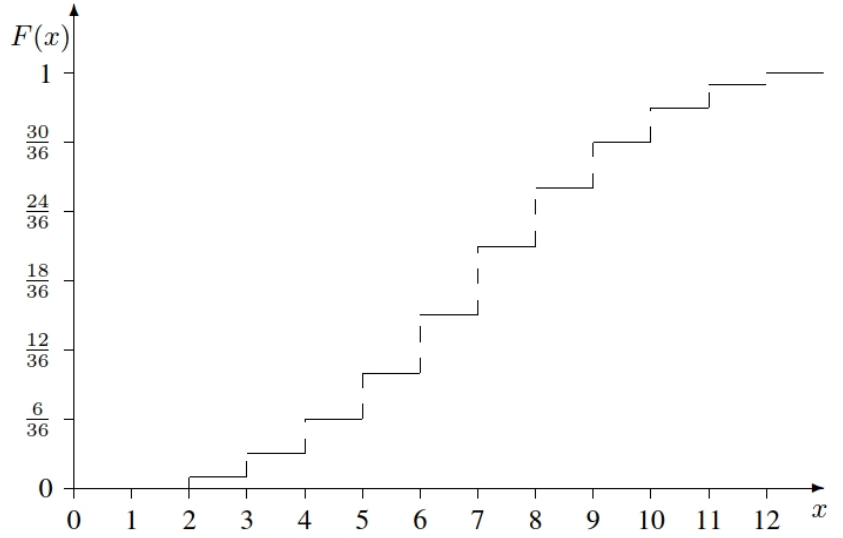
\includegraphics[width=0.2\textwidth]{images/5.2_F_augensumme.png}
    \caption{Wahrscheinlichkeitsion (oben) und Verteilungsfunktion für die Augensummen bei zweimaligen Würfeln.}
    \vspace{-3mm}
    \label{fig:f_F_dice}
\end{wrapfigure}
Bei der Beobachtung oder Durchführung von Zufallsvorgängen ist man häufig gar nicht an den Ergebnissen selbst interessiert, sondern an daraus abgeleiteten Größen. Beim zweimaligen Würfeln könnte dies beispielweise die Summe der Augenzahlen sein. Hier besteht der Ereignisraum $\Omega$ aus 36 Zahlenpaaren $\omega = (i, j)$ mit $1 \le i,j \le 6$, relevant ist für jedes Zahlenpaar aber nur die Information $i + j$. Durch die Zuordnung der reellen Zahl $i + j$ zu jedem Ergebnis $\omega = (i, j)$ erhält man eine \emph{Zufallsvariable}. Wenn wir $X$ für die Augensumme der zwei Würfe verwenden erhalten wir also die Zuordnung bzw. Abbildung $X: \omega = (i, j) X(\omega) = X(i, j) = i + j$. Diese Schreibweise ermöglicht es Ereignisse sehr knapp und einfach zu Formulieren. So entspricht dem Ereignis \glqq die Augensumme ist 4\grqq\, kurz \{$X=4$\} was ausführlich $\{X = 4\} = \{\omega \in \Omega: X(\omega) = 4 = \{(1,3), (2,2), (3,1)\}$ bedeutet. 
\section{Diskrete Zufallsvariablen}
Eine Zufallsvariable heißt diskret, wenn sie nur endlich oder abzählbar unendlich viele Werte annehmen kann, d.h. $W(X) = \{x_1, x_2, ...\}$. Die Wahrscheinlichkeitsverteilung ist dann gegeben durch $P(X = x_i) = p_i$ eindeutig festgelegt. Nach dem ersten Axiom von Kolmogoroff ist $0 \le p_i \le 1$ und die Wahrscheinlichkeit für ein Ereignis $\{X \in A\}$ mit $A \subset W(X)$ ist $P(X \in A) = \sum_{i:x_i \in A} p_i$. Nach dem zweiten Axiom von Kolmogoroff folgt damit sofort $\sum_{i \ge 1} p_i = P(X \in W(X)) = 1$. Die Wahrscheinlichkeitsverteilung ist Analog zur relativen Häufigkeitsverteilung. Während die Wahrscheinlichkeitsverteilung die möglichen Ausgänge eines Zufallsvorgangs theoretisch beschreibt basiert die relative Häufigkeitsverteilung auf tatsächlichen Beobachtungen in einer Stichprobe.
\hlc{Definition Wahrscheinlichkeitsfunktion.}: \hlcm{$f(x) = f_X() := \begin{cases}
    P(X = x_i) = p_i &\text{, }x = x_i \in W(X)\\
    0 &\text{, sonst.}
\end{cases}$}. $W(X)$ sei hierbei der Wertebereich einer Zufallsvariable X.
Die \hlc{Verteilungsfunktion} ist \hlcm{$F(x) = F_X(x) := P(X\le x) = \sum_{i: x_i \le x}f(x_i) = \sum_{i: x_i \le x} p_i$}. Die Verteilungsfunktion ist insbesondere zur \hlc{Berechnung von Wahrscheinlichkeiten der Form $P(a < X \le b)$} mit $a, b \in \mathds{R}$ und $a < b$ hilfreich, denn es gilt \hlcm{$P(a < X \le b) = F(b) - F(a)$}\\\\
\hlc{Unabhänigkeit diskreter Zufallsvariablen}: $n$ Diskrete Zufallsvariablen $X_1, .., X_n$ heißen stochastisch unabhängig, wenn für beliebige $x_1 \in W(X_1), ..., x_n \in W(X_n)$ gilt: $P(X_1 = x_1, ..., X_n = x_n) = P(X_1 = x_1) \cdot ... \cdot P(X_n = x_n)$. Anschaulich: Für das Würfeln von zwei Würfeln  $X_1$ und $X_2$ mit zwei beliebigen Augenzahlen $i$ und $j$ gilt: $P(X_1 = i, X_2 = j) = \frac{1}{36} = \frac{1 \cdot 1}{6 \cdot 6} = P(X_1 = i) \cdot P(X_2 = j)$.

\subsection{Maßzahlen diskreter Wahrscheinlich}
\hlc{Erwartungswert einer Diskreten Zufallsvariable}: Sei $X$ eine diskrete Zufallsvariable mit Wertebereich $W(X) = \{x_1, x_2, ...\}$ und Wahrscheinlichkeitsverteilung $p_1, p_2, ...$. Dann ist der Erwartungswert von $X$:\\ \hlcm{$E(X) := \sum_{i\ge1} x_i \cdot p_i = \sum_{i\ge1} x_i \cdot f(x_i) = \mu_x = \mu$}. Eigenschaften: Für eine Funktion $g: \mathds{R} \rightarrow \mathds{R}$ ist auch $Y = g(X)$ eine Zufallsvariable, und zwar mit Wahrscheinlichkeitsverte\section{\textbf{WAHRSCHEINLICHKEITSTHEORIE} - Ereignisse und Wahrscheinlichkeiten}
\subsection{Zufallsereignisse}
Der Ausgangspunkt jeder wahrscheinlichkeitstheoretischen Betrachtung ist ein Zufallsvorgang oder Zufallsexperiment (Würfeln, prüfen eines Werkstücks). Einen Zufallsvorgang zeichnet aus, dass es mehrere, \emph{sich gegenseitig ausschließende} Ergebnisse gibt, von dem genau eines Eintreten wird, wobei nicht bekannt ist welches. Die \emph{möglichen} Ergebnisse eines Zufallsvorgang werden mit $\omega$ und die Menge aller Ergebnisse d.h. der \emph{Ergebnisraum} werden als $\Omega$ bezeichnet. Beim Einmaligen Würfeln kann $\omega$  z.B. $\omega = \{2\}$ sein, während $\Omega = \{1, 2, 3, 4, 5, 6\}$ ist. Wenn man beim Würfeln eine 5 oder 6 benötigen um zu gewinnen, ist man daran interessiert, ob das
Ergebnis des Würfelwurfes in einer bestimmten Teilmenge von $\Omega$ liegt, konkret in der Menge $\{5, 6\}$. Diese Teilmengen nennt man \emph{(Zufalls-)Ereignisse} und man sagt, dass ein Ereignis $A \subset \Omega$ eintritt, wenn das Ergebnis $\omega$ des Zufallsvorgang ein Element von A is. Die einelementigen Teilmengen $\{\omega\}$ von $\Omega$ nennt man auch \emph{Elementareereignisse}.\\\\
\textbf{Mengenlehre und wahrscheinlichkeitstheoretische Interpretation}: \emph{Kommutativgesetz}: $A \cap  B = B \cap A$. \emph{Assoziativgesetz}: $(A \cap B ) \cap C = A \cap (B \cap C)$. \emph{Distributivgesetz}: $(A \cup B) \cap C = (A \cap C) \cup (A \cap C)$. \emph{De Morgansche Regel}: $\overline{(A \cap B)} = \bar{A} \cup \bar{B}$ (geht auch, wenn man $\cap$ und $\cup$ vertauscht)\\\\
\textbf{Ereignisfelder}: Die Menge aller Ergebnisse bezeichnet man als \emph{Ereignisfeld} $\mathcal{F}$. Wenn der Ergebnisraum $\Omega$ endlich oder abzählbar unendlich ist, ist die Potenzmenge $\mathcal{P}(\Omega)$ das üblicherweise betrachtete Ereignisfeld. Ist $\Omega$ überabzählbar können als Ereignisfelder nur $\sigma$-Algebren betrachtet werden. Diese sind definiert durch: $\Omega \in \mathcal{F}$,\,\,\,$A \in \mathcal{F} \Rightarrow \bar{A} \in \mathcal{F}$,\,\,\,abzählbar viele Ereignisse $A_1, A_2, ... \in \mathcal{F} \Rightarrow \cup_{i=1}^\infty A_i \in \mathcal{F}$

\subsection{Laplace-Wahrscheinlichkeiten und Kombinatorik}
\begin{wrapfigure}{r}{0.4\textwidth}
    \vspace{-6mm}
    \centering
    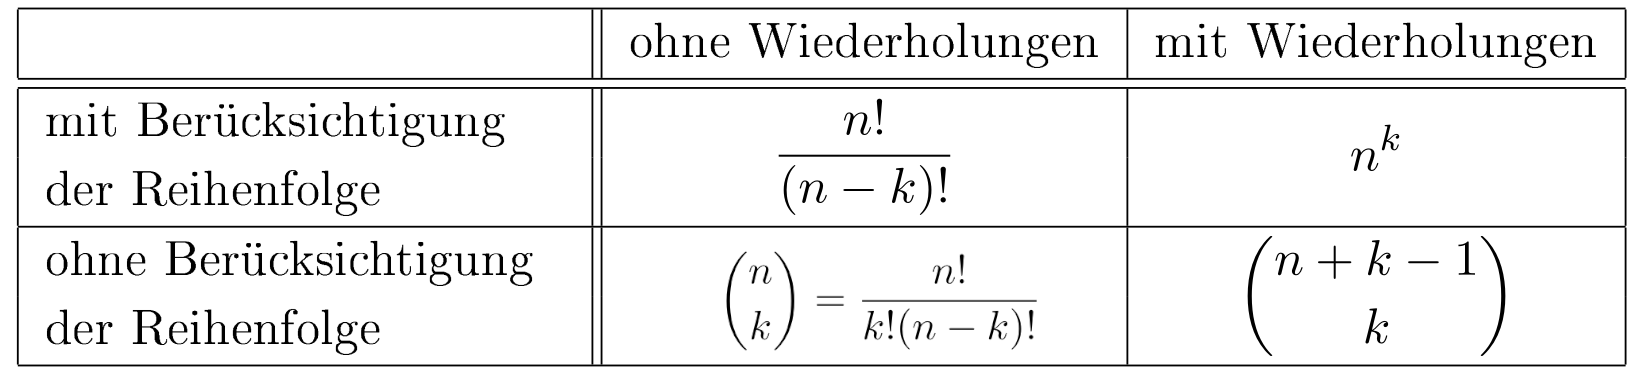
\includegraphics[width=0.4\textwidth]{images/wiederholung_kombinatorik.png}
    \caption{Kombinatorik Wiederholung}
    \vspace{-6mm}
    \label{fig:}
\end{wrapfigure}
\textbf{Laplace-Wahrscheinlichkeit}: $P(A) = \frac{\text{Anzahl der für $A$ günstigen Ergebnisse}}{\text{Anzahl aller möglichen Ergebnisse}} = \frac{|A|}{|\Omega|}$. Bsp. die Wahrscheinlichkeit eine ungerade Zahl zu würfeln: $P(A) = \frac{|\{1,3,5\}|}{|\{1,2,3,4,5,6\}|} = \frac{3}{6} = \frac{1}{2}$

\textbf{Permutation}: Anordnen von n unterscheidbaren Objekten: $n \cdot (n-1) \cdot (n-2) ... = \Pi_{i=1}^n i = n!$. Bsp: Sitzordnung an einem Tisch.\,\,\,\,\textbf{Variation ohne Wiederholungen}: Möglichkeiten k aus n unterscheidbaren Objekten \emph{mit} Berücksichtigung der Reihenfolge auszuwählen. Formel 1 Siegertreppchen Anordnungen bei 20 Teilnehmern.\,\,\,\,\textbf{Variation mit Wiederholungen}: Bsp. k mal ziehen aus n Möglichkeiten. Bsp: Kombinationen bei Passwörtern.\,\,\,\,\textbf{Kombination ohne Wiederholungen} Ziehen von k aus n Objekten. Die Reihenfolge spielt keine Rolle. Bsp: \hlc{Lotto} 6 aus 49.\,\,\,\,\textbf{Kombination mit Wiederholungen}: Die Anzahl Kombinationen beim Auswählen von k Objekten aus n unterscheidbaren Objekten.
\subsection{Wahrscheinlichkeitsmaße}
\textbf{Definition Wahrscheinlichkeitsmaß}: Es sei $\Omega$ der Ergebnisraum eines Zufallsvorgangs und $\mathcal{F}$ ein Ereignisfeld über $\Omega$. Eine Abbildung $P$ die jedem Ereignis $A \in \mathcal{F}$ eine reelle Zahl zuordnet: $P: \mathcal{F} \rightarrow \mathds{R}$ mit $A \mapsto P(A)$ nennt man \emph{Wahrscheinlichkeitsmaß} auf $\mathcal{F}$ wenn sie die \hlc{Axiome von Kolmogoroff} erfüllt: \textbf{K1} $P(A) \ge 0$ (Nichtnegativität).\,\,\,\,\textbf{K2} $P(\Omega) = 1$ (Normierung).\,\,\,\,\textbf{K3} Falls $A \cap B = \emptyset$, so ist $ (A \cup B) = P(A) + P(B)$ (Additivität).\\
Daraus folgen folgende Rechenregel:\,\,\,\,(\textbf{i}) $0 \le P(A) \le 1$.\,\,\,\,(\textbf{ii}) $P(\emptyset) = 0$.\,\,\,\,(\textbf{iii}) $P(A) \le P(B)$, falls $A \subset B$.\,\,\,\,(\textbf{iv}) $P(\bar{A}) = 1 - P(A)$.\,\,\,\,(\textbf{v}) $P(A_1\cup ... \cup A_k) = P(A_1) + ... + P(A_k)$ falls $A_1, ..., A_k$ paarweise disjunkt. $\Rightarrow$ $P(A) = \sum_{w \in A}P(\{\omega\}.$\,\,\,\,(\textbf{vi}) $P(B \backslash A) = P(B) - P(A \cap B)$.\,\,\,\,(\textbf{vii}) $P(A\cup B) = P(A) + P(B) - P(A \cap B)$ (Additionssatz)
\subsection{Bedingte Wahrscheinlichkeiten und unabhängige Ereignisse}
Die Wahrscheinlichkeit eines Ereignisses ändert sich möglicherweise, wenn wir zusätzlich Information in Form des Eintritts eines anderen Ereignisses erhalten. Wahrscheinlichkeit für Pünktlichkeit sinkt bei Stau. Die Definition der \hlc{bedingten Wahrscheinlichkeit} ergibt sich hierbei Analog zur relativen Häufigkeitsverteilung: \hlcm{$P(A|B) = \frac{P(A \cap B)}{P(B)}$}. Bsp: Wie hoch ist die Wahrscheinlichkeit eine 6 zu würfeln unter der Bedingung, dass die gewürfelte Zahl gerade ist? Antwort: $P(A|B) = \frac{P(\{6\} \cap \{2,4,6\})}{P(\{2,4,6\})} = \frac{1/6}{3/6} = \frac{1}{3}$\\
\begin{wrapfigure}{l}{0.25\textwidth}
    \vspace{-6mm}
    \centering
    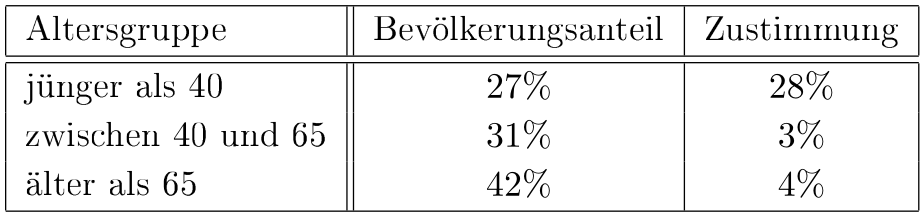
\includegraphics[width=0.25\textwidth]{images/beispiel_wahl_satz_der_tot_wahscheinlichkeit.png}
    \caption{Eine Partei hat analysiert, wie ihre Demographie ist.}
    \vspace{-5mm}
    \label{fig:pool_total}
\end{wrapfigure}
Der \hlc{Produktsatz} garantiert, dass für zwei Ergebnisse $A$ und $B$ mit $P(B) > 0$ gilt: \hlcm{$P(A \cap B) = P(B) \cdot P(A|B)$}. Diese Aussage gilt auch im allgemeinen für $A_1, ..., A_n$ mit $P(A_1 \cap ... \cap A_n) > 0$:\\$P(\cap_{i=1}^nA_i) = P(A_1) \cdot P(A_2|A_1) \cdot P(A_3|A_1 \cap A_2) \cdot P(A_n|A_1 \cap ... \cap A_{n-1}) = P(A_1) \cdot \Pi_{i=2}^n P(A_i|A_1 \cap ... \cap A_{i-1})$. \hlc{Stochastiche Unabhängikeit} bedeutet wenn sich die Wahrscheinlichkeit eines Ereignisses $A$ beim Eintritt eines anderen Ereignisses $B$ \emph{nicht} ändert. Sprich $P(A|B) = P(A)$. Somit gild dann mit dem Produktsatz $P(A \cap B) = P(B) \cdot P(A | B) = P(B) \cdot P(A)$. Dies gilt Analog für $n$ Ereignisse. \hlc{Satz der totalen Wahrscheinlichkeit}: Sei $A_1, ..., A_n$ eine disjunkte Zerlegung des Ereignisraums $\omega$ mit $P(A_j) > 0$, $j = 1, ..., n$. Dann gilt für ein weiteres Ereignis $B$: \hlcm{$P(B) = \sum_{j=1}^nP(B|A_j) \cdot P(A_j)$}. Bsp Wahl (vgl \cref{fig:pool_total}) Welchen Stimmanteil hat die Partei insgesamt bekommen? Antwort: $P(B) = \sum_{j=1}^3 = P(B|A_j) \cdot P(A_j) = 0.28 \cdot 0.27 + 0.03 \cdot 0.031 + 0.04 \cdot 0.42 = 0.1017$. \hlc{Satz von Bayes}: Sei $A_1, ..., A_n$ eine disjunkte Überdeckung des Ereignisses $B$ und $P(A_j) > 0$ sowie $P(B|A_j) > 0$ für mindestens ein $j = 1, ..., n$. Dann gilt: \hlcm{$P(A_j|B) = \frac{P(B|A_j) \cdot P(A_j)}{P(B)} = \frac{P(B|A_j) \cdot P(A_j)}{\sum_{i=1}^nP(B|A_i) \cdot P(A_i)}, j = 1, ..., n$}. Dieser Satz überträgt die \emph{a-priori} Wahrscheinlichkeit $P(A_j)$ in eine \emph{a-posteriori} Wahrscheinlichkeit $P(A_j|B)$. Bsp. Wie groß ist die Wahrscheinlichkeit, dass ein Wähler zur Gruppe \glqq jünger als 40\grqq\, gehört? Antwort: ($P(B)$ wurde mit Satz der tot. Wahrscheinlichkeit berechnet) $P(A_1|B) = \frac{P(B|A_1) \cdot P(A_1)}{P(B)} = \frac{0.28 \cdot 0.27}{0.1017}$
\section{Zufallsvariablen}
\begin{wrapfigure}{r}{0.2\textwidth}
    \vspace{-10mm}
    \centering
    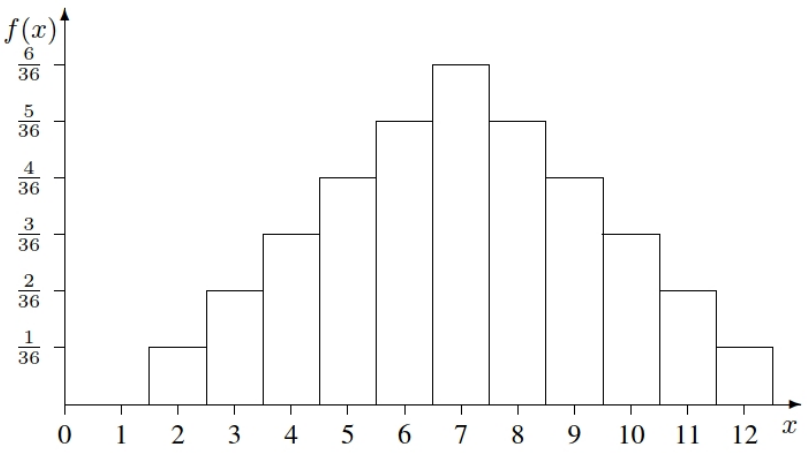
\includegraphics[width=0.2\textwidth]{images/5.1_f_augensumme.png}
    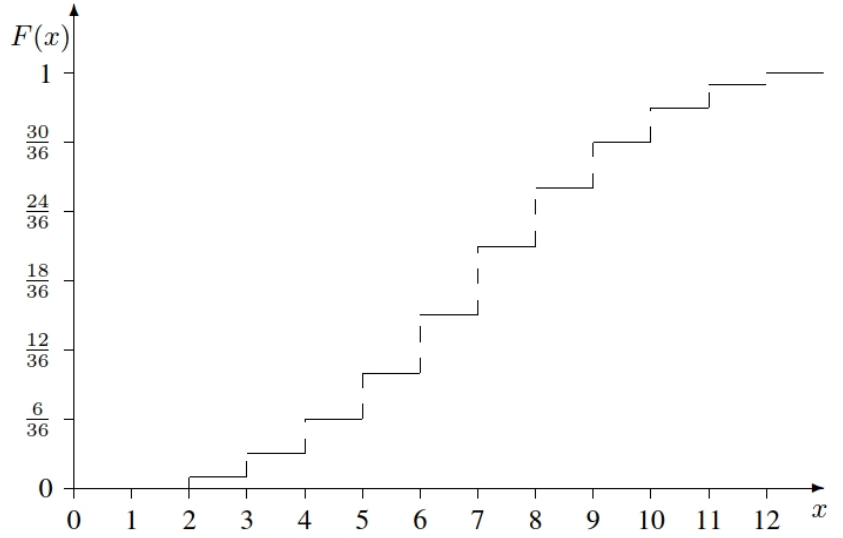
\includegraphics[width=0.2\textwidth]{images/5.2_F_augensumme.png}
    \caption{Wahrscheinlichkeitsion (oben) und Verteilungsfunktion für die Augensummen bei zweimaligen Würfeln.}
    \vspace{-3mm}
    \label{fig:f_F_dice}
\end{wrapfigure}
Bei der Beobachtung oder Durchführung von Zufallsvorgängen ist man häufig gar nicht an den Ergebnissen selbst interessiert, sondern an daraus abgeleiteten Größen. Beim zweimaligen Würfeln könnte dies beispielweise die Summe der Augenzahlen sein. Hier besteht der Ereignisraum $\Omega$ aus 36 Zahlenpaaren $\omega = (i, j)$ mit $1 \le i,j \le 6$, relevant ist für jedes Zahlenpaar aber nur die Information $i + j$. Durch die Zuordnung der reellen Zahl $i + j$ zu jedem Ergebnis $\omega = (i, j)$ erhält man eine \emph{Zufallsvariable}. Wenn wir $X$ für die Augensumme der zwei Würfe verwenden erhalten wir also die Zuordnung bzw. Abbildung $X: \omega = (i, j) X(\omega) = X(i, j) = i + j$. Diese Schreibweise ermöglicht es Ereignisse sehr knapp und einfach zu Formulieren. So entspricht dem Ereignis \glqq die Augensumme ist 4\grqq\, kurz \{$X=4$\} was ausführlich $\{X = 4\} = \{\omega \in \Omega: X(\omega) = 4 = \{(1,3), (2,2), (3,1)\}$ bedeutet. 
\section{Diskrete Zufallsvariablen}
Eine Zufallsvariable heißt diskret, wenn sie nur endlich oder abzählbar unendlich viele Werte annehmen kann, d.h. $W(X) = \{x_1, x_2, ...\}$. Die Wahrscheinlichkeitsverteilung ist dann gegeben durch $P(X = x_i) = p_i$ eindeutig festgelegt. Nach dem ersten Axiom von Kolmogoroff ist $0 \le p_i \le 1$ und die Wahrscheinlichkeit für ein Ereignis $\{X \in A\}$ mit $A \subset W(X)$ ist $P(X \in A) = \sum_{i:x_i \in A} p_i$. Nach dem zweiten Axiom von Kolmogoroff folgt damit sofort $\sum_{i \ge 1} p_i = P(X \in W(X)) = 1$. Die Wahrscheinlichkeitsverteilung ist Analog zur relativen Häufigkeitsverteilung. Während die Wahrscheinlichkeitsverteilung die möglichen Ausgänge eines Zufallsvorgangs theoretisch beschreibt basiert die relative Häufigkeitsverteilung auf tatsächlichen Beobachtungen in einer Stichprobe.
\hlc{Definition Wahrscheinlichkeitsfunktion.}: \hlcm{$f(x) = f_X() := \begin{cases}
    P(X = x_i) = p_i &\text{, }x = x_i \in W(X)\\
    0 &\text{, sonst.}
\end{cases}$}. $W(X)$ sei hierbei der Wertebereich einer Zufallsvariable X.
Die \hlc{Verteilungsfunktion} ist \hlcm{$F(x) = F_X(x) := P(X\le x) = \sum_{i: x_i \le x}f(x_i) = \sum_{i: x_i \le x} p_i$}. Die Verteilungsfunktion ist insbesondere zur \hlc{Berechnung von Wahrscheinlichkeiten der Form $P(a < X \le b)$} mit $a, b \in \mathds{R}$ und $a < b$ hilfreich, denn es gilt \hlcm{$P(a < X \le b) = F(b) - F(a)$}\\\\
\hlc{Unabhänigkeit diskreter Zufallsvariablen}: $n$ Diskrete Zufallsvariablen $X_1, .., X_n$ heißen stochastisch unabhängig, wenn für beliebige $x_1 \in W(X_1), ..., x_n \in W(X_n)$ gilt: $P(X_1 = x_1, ..., X_n = x_n) = P(X_1 = x_1) \cdot ... \cdot P(X_n = x_n)$. Anschaulich: Für das Würfeln von zwei Würfeln  $X_1$ und $X_2$ mit zwei beliebigen Augenzahlen $i$ und $j$ gilt: $P(X_1 = i, X_2 = j) = \frac{1}{36} = \frac{1 \cdot 1}{6 \cdot 6} = P(X_1 = i) \cdot P(X_2 = j)$.

\subsection{Maßzahlen diskreter Wahrscheinlich}
\hlc{Erwartungswert einer Diskreten Zufallsvariable}: Sei $X$ eine diskrete Zufallsvariable mit Wertebereich $W(X) = \{x_1, x_2, ...\}$ und Wahrscheinlichkeitsverteilung $p_1, p_2, ...$. Dann ist der Erwartungswert von $X$:\\ \hlcm{$E(X) := \sum_{i\ge1} x_i \cdot p_i = \sum_{i\ge1} x_i \cdot f(x_i) = \mu_x = \mu$}. Eigenschaften: \textbf{1} Für eine Funktion $g: \mathds{R} \rightarrow \mathds{R}$ ist auch $Y = g(X)$ eine Zufallsvariable, und zwar mit Wahrscheinlichkeitsverteilung $P(Y = y) = \sum_{i: g(x_i) = y} p_i$. \textbf{2} Der Erwartungswert von $Y$ ist dann $E(Y) = E(g(X)) = \sum_{i\ge1} g(x_i) \cdot p_i = \sum_{i\ge1} g(x_i) f(x_i)$. \textbf{3} Im Spezialfall einer linearen Transformation $g(x) = ax + b$ ist $E(Y) = E(aX+b) = aE(X) + b$. \textbf{4} Für Zufallsvariablen $X_1, ..., X_n$ und Konstanten $a_1, ..., a_n \in \mathds{R}$ gilt $E(a_1X_1 + ... + a_nX_n) = a_1E(X_1) + ... + a_nE(X_n)$. \textbf{5} Für unabhängige Zufallsvariablen $X_1$ und $X_2$ gilt außerdem $E(X_1 \cdot X_2) = E(X_1) \cdot E(X_2)$\\\\
\hlc{Modus disktrer Zufallsvariablen} Jede lokale Maximumstelle der Wahrscheinlichkeitsfunktion $f_X(x)$ einer diskreten Zufallsvariablen $X$ ist ein Modus $x_{mod}$ der Verteilung von $X$. Bsp. Lokales Maximum in \cref{fig:f_F_dice} (oben) ist $x_mod$.\\\\
\hlc{Varianz und Standardabweichung diskreter Zufallsvariablen} Sei $X$ eine diskrete Zufallsvariable mit Wertebereich $W(X) = \{x_1, x_2, ...\}$ und Wahrscheinlichkeitsverteilung $p_1, p_2$. dann ist die Varianz von $X$: $\sigma_x^2 = \sigma^2 = Var(X):= $ $ :=\sum_{i\ge1} (x_i - E(X))^2 \cdot p_i = \sum_{i\ge1} = (x_i - E(X))^2 \cdot f(x_i)$ dementsprechend ist die Varianz \hlcm{$\sigma = \sqrt{Var(X)}$}. Bei der praktischen Berechnung ist der \emph{Verschiebungssatz} recht hilfreich: \hlcm{$Var(X) = E(X^2) - (E(X))^2$}. Eigenschaften der Varianz: \textbf{1} Die Varianz der transformierten Y(X) = g(X) als reelle Funktion ist $Var(Y) = Var(g(X)) = \sum_{i\ge1} [g(x_i) - E(g(X))]^2 \cdot p_i = \sum_{i\ge1} [g(x_i) - E(g(X))]^2 \cdot f(x_i) = E[(g(X) - E(g(X)))^2] = E(g(X)^2) - E^2(g(X))$. \textbf{2} Im Spezialfall einer lin. Transformation $g(x) = ax + b$  ist $Var(Y) = Var(aX + b) = a^2Var(X)$ damit folgt für die Stdabw. $\sigma_Y = |a|\sigma_x$. \textbf{3} Für unabhängige Zufallsvariablen $X_1, ..., X_n$ und Konst. $a_1, ..., a_n \in \mathds{R}$ gilt: $Var(a_1X_1 + ... + a_nX_n) = a_1^2Var(X_1) + ... + a_n^2Var(X_n)$ 
\subsection{Konkrete diskrete Wahrscheinlichkeitsverteilungen}
\hlc{Diskrete Gleichverteilung} Eine diskrete Zufallsvariable heißt gleich- oder Laplace-verteilt, wenn alle möglichen Werte mit gleicher Wahrscheinlichkeit auftreten. Wahrscheinlichkeitsfunktion: $f(x) = \begin{cases}
    \frac{1}{n}&x\in W(X)\\
    0&\text{sonst}
\end{cases}$. Erwartungswert: $E(X) = \frac{1}{n}\sum_{i=1}^nx_i$. Varianz: $Var(X) = E(X^2) - (E(X))^2 = \frac{1}{n}\sum_{i=1}^nx_i^2 - \frac{1}{n^2}(\sum_{i=1}^nx_i)^2$. \emph{Mögliche Anwendungen:} Münzwurf, Würfel. \\\\
\hlc{Bernoulli-Verteilung - $X \sim Ber(p)$}: Einen Zufallsvorgang, der nur zwei mögliche Ergebnisse hat. In der Regel geht es um die Frage, ob ein bestimmtes Ereignis A eintritt oder nicht. $W(X) = \{0,1\}$. \hlc{$p = P(A)$}. Wahrscheinlichkeitsverteilung: $p_0 = P(X=0) = 1 - p$ und $p_1 = P(X=1) = p$. $E(X) = p$ und $Var(X) = p(1-p)$. \emph{Mögliche Anwendungen:} Qualitätsprüfung (Bauteil besteht oder nicht)\\\\
\hlc{Binomialverteilung - $X \sim Bin(n, p)$ / $X \sim B(n, p)$} Erweiterung der Bernoulli-Verteilung. Man führt ein Bernoulli-Experiment \hlc{$n$}-Mal durch. Wahrscheinlichkeit für $k$ von $n$ erfolgreiche Versuche: $p_k = \binom{n}{k} p^k  (1-p)^{n-k}, k = 0, ..., n$. Wahrscheinlichkeitsfunktion $f(X) = P(X = x) = \begin{cases}
    \binom{n}{x} p^x  (1-p)^{n-x} & x = 0, 1, ..., n\\
    0 & \text{sonst}
\end{cases}$. Erwartungswert $E(X) = np$. $Var(X) = np(1-p)$. Gilt $X \sim Bin(n, p)$ und $Y \sim Bin(m, p)$ so gilt $X + Y \sim Bin(n + m, p)$. \emph{Mögliche Anwendungen:} Modellierung der Wahrscheinlichkeit, dass ein Byte Korrekt übertragen wird.\\\\
\hlc{Poisson-Verteilung - $X \sim Poi(\lambda)$} Modelliere Anzahl von Ereignissen in begrenzten Zeitraum. $W(X) = \mathds{N}_0$. Annahmen: \textbf{1} Zwei Ereignisse können nicht gleichzeitig auftreten. \textbf{2} Die Wahrscheinlichkeit für ein Ereignis Wächst proportional mit der Länge des betrachteten Zeitabschnitts. \textbf{3} Die \emph{Wahrscheinlichkeit} für eine bestimmte Anzahl Ereignisse hängt nur von der Länge des betrachteten Zeitintervalls ab, nicht von dessen Lage. Für tatsächliche Beobachtungen gilt das natürlich nicht. \textbf{4} Die Anzahl von Ereignissen in zwei disjunkten Zeitintervallen sind unabhängig. Wahrscheinlichkeitsfunktion: $f(x) = P(X=x) = \begin{cases}
    \frac{\lambda^x}{x!}e^{-\lambda} & x \in \mathds{N}_0\\
    0 & text{sonst}
\end{cases}$. $E(X) = \lambda$ $Var(X) = \lambda$. $X \sim Poi(\lambda)$ und $Y \sim Poi(\mu)$ $\Rightarrow$ $X + Y \sim Poi(\lambda + \mu)$ \emph{Mögliche Anwendungen} Reaktorüberwachung. 5 Ereignisse pro Tag. Wie hoch ist die Wahrscheinlichkeit für mehr als Zehn? $\rightarrow$ $P(N > 10) = \sum_{k=11}^\infty p_k = 1 - \sum_{k=0}^{10}p_k$ \\\\
\hlc{Geometrische Verteilung - $Geo(p)$} Zum modellieren der Anzahl an notwendiger Wiederholungen bis zum erstmaligen Eintritt des erwarteten Ereignisses. Sei $X$ die Anzahl \emph{unabhängiger} Versuchswiederholungen bis zum erstmaligen Eintritt des Ergebnisses $A$ und \hlc{$p = P(A)$}. Die Wahrscheinlichkeitsfunktion lautet $f(X) = P(X = x) = \begin{cases}
    (1 - p) ^ (k-1) p & x \in \mathds{N}\\
    0 & \text{sonst}
\end{cases}$. $E(X) = \frac{1}{p}$. $Var(X) = \frac{1-p}{p^2}$. Außerdem Verteilungsfunktion für $x \ge 0$: $F(x) = P(X \le x) = P(X \le \lfloor x\rfloor) = 1 - (1 - p)^{\lfloor x\rfloor}$



\section{Stetige Zufallsvariablen}
\section{Gesetz der großen Zahlen und zentraler Grenzwertsatz}
\section{Zufallsvektoren}

